\documentclass[11pt,a4paper,oneside]{article}
\usepackage{amsmath}
\usepackage{listings}
\usepackage[utf8]{inputenc}
\usepackage[T1]{fontenc}
\usepackage{color}
\usepackage[icelandic]{babel}
\usepackage{enumerate}
\usepackage{graphicx}
\usepackage{wrapfig}
\usepackage{titling}
\newcommand{\subtitle}[1]{%
  \posttitle{%
    \par\end{center}
    \begin{center}\large#1\end{center}
    \vskip0.5em}%
}

\newcommand{\problemstatement}[1]{ \input #1.tex }

\title{Forritunarkeppni Framhaldsskólanna 2013}
\subtitle{Kirk deild}
\date{16. mars 2013}
\author{Háskólinn í Reykjavík}

\begin{document}

	\maketitle
	\thispagestyle{empty}
	\pagebreak

	\section*{Candy Crush}

	Í þessu verkefni á að útfæra leikinn Candy Crush. Leikurinn Candy Crush er spilaður á ferhyrndu leikborði af ákveðinni stærð. Til eru nokkrar mismunandi gerðir af nammi, og er eitt nammi á hverjum reit á leikborðinu. Ef þrjú eða fleiri nammi af sömu gerð liggja saman í röð, þá hverfa reitirnir sem þau nammi voru á, og reitirnir fyrir ofan hliðrast niður á við og hylja þannig gapið sem myndaðist. Leikmaður má víxla á tveimur samliggjandi reitum, og þar með fært nammi af sömu gerð hlið við hlið.

	\begin{figure}[h]
		\centering
		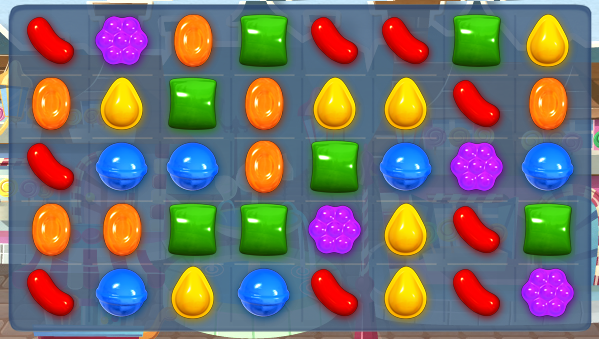
\includegraphics[scale=0.8]{candycrush.png}
	\end{figure}

	\subsection*{Grunnkröfur}
	Eftirfarandi grunnkröfur er \textbf{nauðsynlegt} að útfæra.

	\begin{itemize}
		\item Ferhyrnt leikborð búið til með nammi í hverjum reit af handahófi.
		\item Hægt að framkvæma hreyfingar, þ.e. víxla á tveimur samliggjandi reitum.
			\begin{itemize}
				\item Ef að hreyfing veldur því að þrír eða fleiri eins reitir myndi röð eða dálk, þá hverfa þeir reitir og aðrir reitir í kring hliðrast niður á við til að fylla upp í þá reiti sem hurfu.
				\item Auðir reitir sem myndast í efstu reitum eru fylltir með nammi af handahófi.
				\item Hreyfing er aðeins lögleg ef hún veldur því að þrír eða fleiri eins reitir myndi röð eða dálk.
				\item Ólöglegar hreyfingar hafa engin áhrif á leikborðið.
			\end{itemize}
		\item Leikmaður fær stig fyrir löglegar hreyfingar og leikmaður hefur takmarkaðan fjölda hreyfinga.
		\item Leik lýkur þegar leikmaður hefur náð settum stigafjölda eða þegar leikmaður hefur notað allar hreyfingar.
		\item Ef að borðið kemst í þá stöðu að engir löglegir leikir eru mögulegir, þá er reitunum endurraðað þannig að a.m.k. ein lögleg hreyfing sé möguleg.
	\end{itemize}

	Hér á eftir koma hugmyndir að aukinni virkni leiksins.

	\subsection*{Spilun}

	\begin{itemize}
		\item Gera grafískt viðmót fyrir leikinn.
		\item Mismunandi stærðir af leikborðum, eða mismunandi lögun af leikborðum (ekki bara ferhyrnd).
		\item Breytilegur fjöldi nammitegunda.
		\item Hafa önnur markmið en að ná lágmarks stigafjölda. T.d. fjarlægja sérstakar tegundir reita, eða öll nammi af ákveðinni tegund.
		\item Hafa bónusnammi sem eyða heilum röðum eða dálkum, eða nammi innan ákveðinnar fjarlægðar eða fjarlægja öll nammi af ákveðinni tegund.
		\item Útfæra fleiri en eitt borð (stig). Notandi getur þá klárað fyrsta borð, og þar með komist á annað borð, og svo framvegis. Mismunandi borð geta haft mismunandi markmið.
		\item Hafa hljóð í leiknum (tónlist og hljóðbrellur).
		\item Útfæra "`undo"' á hreyfingar.
			\begin{itemize}
				\item Leikmaður getur afturkallað síðustu hreyfingar og komið borðinu í þá stöðu sem það var áður en hreyfingunum var beitt.
			\end{itemize}
	\end{itemize}

	\subsection*{Gagnagrunnur}

	\begin{itemize}
		\item Útfæra notendakerfi.
		\item Geyma upplýsingar um leikmenn
			\begin{itemize}
				\item Leikjasögu, þ.e. geyma fyrir sérhvern leik sem leikmaður spilar hvaða borð hann var að spila, hversu mörg stig hann fékk, o.s.frv.
				\item Hvaða borð hefur leikmaður unnið.
				\item Hvaða vinninga hann hefur unnið sér inn.
			\end{itemize}
		\item Geta birt upplýsingar
			\begin{itemize}
				\item Efstu leikmenn (sem hafa flest stig).
				\item Sögu hvers leikmanns
					\begin{itemize}
						\item Hversu marga leiki hefur hann unnið.
						\item Frammistaða í hverju borði.
						\item Hvaða vinninga hann hefur náð sér í.
					\end{itemize}
			\end{itemize}
		\item Geyma upphafsstöðu og allar hreyfingar úr öllum leikjum í gagnagrunni.
			\begin{itemize}
				\item Bjóða upp á að fá að horfa á endurspilun á eigin leikjum og leikjum annarra.
			\end{itemize}
	\end{itemize}

	\subsection*{Netsamskipti}
		\begin{itemize}
			\item Búa til miðlara (e. server) sem að gerir tveimur, eða fleiri, leikmönnum kleift að spila leikinn samtímis.
			\item Leikmenn geta spilað leikinn í sameiningu eða geta spilað á móti hvorum öðrum.
			\item Leikmenn geta spjallað saman.
			\item Leikmenn hittast í anddyri (e. lobby)
				\begin{itemize}
					\item Geta spjallað saman í anddyrinu.
					\item Geta óskað eftir að spila leik við aðra leikmenn.
				\end{itemize}
		\end{itemize}


\end{document} 